\section{Decodificação da Instrução}
	\subsection{Diagrama de Classe}
  \begin{figure}[htpb!]
    \begin{center}
	\begin{tikzpicture}
	\umlclass[x=0,y=0]{Instruction Decode}{
	+ clock : input bit \\
	+ reset : input bit \\
	+ instruction : input bit[32] \\ 
	+ regDst : input bit \\
	+ writeData : input bit \\
	+ writeRegister : input bit \\
	+ word : input bit[16] \\
	+ regDst : output bit \\
	+ branch : output bit \\
	+ memRead : output bit \\
	+ memToReg : output bit \\
	+ aluOp : output bit \\
	+ memWrite : output bit \\
	+ aluSrc : output bit \\
	+ regWrite : output bit \\
	+ jump : output bit \\
	+ readData1 : output bit[32] \\
	+ readData2 : output bit [32] \\
	+ outputWord : output bit [32] \\
	+ registers : reg bit[32] \\}			
	{ % procedures
          - \underline{<<comb>> opcode\_decoder()} \\
          - <<comb>> search\_register() \\
          - <<comb>> set\_write\_register() \\
          - <<sequ>> sign\_extend() \\
          - <<sequ>> zero\_extend()
        }
	\end{tikzpicture}
\end{center}
  \end{figure}
		
		\subsection{Definições de entrada e saída}
		
	\begin{center}
		\begin{longtable}[pos]{| l | c | c | m{7cm} |} \hline
			\multicolumn{1}{|c|}{\cellcolor[gray]{0.9}\textbf{Nome}} & 
			\multicolumn{1}{c|}{\cellcolor[gray]{0.9}\textbf{Tamanho}} & 
			\multicolumn{1}{c|}{\cellcolor[gray]{0.9}\textbf{Direção}} &
			\multicolumn{1}{c|}{\cellcolor[gray]{0.9}\textbf{Descrição}} \\ \hline
			\endhead
			\hline
			\endlastfoot
			
			clock & 1 & entrada & Clock do sistema \\ \hline
			reset & 1 & entrada & Sinal de reinício do estágio\\ \hline
			instruction & 32 & entrada & Instrução a ser executada. \\ \hline
			writeData & 1 & entrada & Sinal de controle para escrita no registrador. \\ \hline
			writeRegister & 5 & entrada & Endereço do registrador de destino do writeData. \\ \hline
			word & 16 & entrada & Os primeiros 16 bits da instrução \\ \hline
			branch & 1 & saída & Sinal que informa ao circuito se a instrução é de branch. \\ \hline
			memRead & 1 & saída & Sinal de controle para realizar leitura da memória. \\ \hline
			memToReg & 1 & saída & Sinal de controle que define se o dado deve vir da ULA ou da memória \\ \hline
			aluOp & 2 & saída & Sinal de controle que define se o campo \textit{funct} da instrução deve ser levado em consideração ou não. \\ \hline
			memWrite & 1 & saída & Sinal de controle para realizar escrita na memória. \\ \hline
			aluSrc & 1 & saída & Sinal de controle que define qual entrada a ULA deve utilizar para realizar a operação. \\ \hline
			regWrite & 1 & saída & Sinal de controle para realizar escrita no registrador. \\ \hline
			jump & 1 & saída & Sinal que informa ao circuito se a operação é de jump. \\ \hline
		\end{longtable}
	\end{center}
    
    		\subsection{Tabela de microinstruções}

	\begin{center}
		\begin{longtable}[pos]{| c | c |} \hline
			\multicolumn{1}{|c|}{\cellcolor[gray]{0.9}\textbf{Código}} & 
			\multicolumn{1}{c|}{\cellcolor[gray]{0.9}\textbf{Instrução}} \\ \hline 
			\endhead
			\hline
			\endlastfoot
			
	    	1 & Lógicas, Aritméticas, MUL e DIV\\ \hline
            2 & ADDI \\ \hline
            3 & ANDI \\ \hline
            4 & SUBI \\ \hline
            5 & ORI \\ \hline
            6 & SW \\ \hline
            7 & LW \\ \hline
            8 & JR\\ \hline
            9 & JPC\\ \hline
            10 & BRFL\\ \hline
            11 & CALL\\ \hline
            12 & RET\\ \hline
            13 & HALT\\ \hline
            14 & NOP\\ \hline
            15 & CMP\\ \hline
		\end{longtable}
	\end{center}

	\begin{center}
		\begin{longtable}[pos]{| c | c | c | c | c | c | c | c | c | c | c | c | c | c | c | c | c |} \hline
			\multicolumn{1}{|c|}{\cellcolor[gray]{0.9}\textbf{\small Código}} & 
			\multicolumn{1}{c|}{\cellcolor[gray]{0.9}\textbf{1}} & 
			\multicolumn{1}{c|}{\cellcolor[gray]{0.9}\textbf{2}} &
			\multicolumn{1}{c|}{\cellcolor[gray]{0.9}\textbf{3}} &
            \multicolumn{1}{c|}{\cellcolor[gray]{0.9}\textbf{4}} &
            \multicolumn{1}{c|}{\cellcolor[gray]{0.9}\textbf{5}} &
            \multicolumn{1}{c|}{\cellcolor[gray]{0.9}\textbf{6}} &
            \multicolumn{1}{c|}{\cellcolor[gray]{0.9}\textbf{7}} &
            \multicolumn{1}{c|}{\cellcolor[gray]{0.9}\textbf{8}} &
            \multicolumn{1}{c|}{\cellcolor[gray]{0.9}\textbf{9}} &
            \multicolumn{1}{c|}{\cellcolor[gray]{0.9}\textbf{10}} &
			\multicolumn{1}{c|}{\cellcolor[gray]{0.9}\textbf{11}} &
			\multicolumn{1}{c|}{\cellcolor[gray]{0.9}\textbf{12}} &
            \multicolumn{1}{c|}{\cellcolor[gray]{0.9}\textbf{13}} &
            \multicolumn{1}{c|}{\cellcolor[gray]{0.9}\textbf{14}} &
            \multicolumn{1}{c|}{\cellcolor[gray]{0.9}\textbf{15}} \\ \hline
			\endhead
			\hline
			\endlastfoot
			
			\small regDst 			& 1   & 0   & 0   & 0   & 0   & 0   & 0   & 0   & 0   & 0   & 0   & 0   & 0  & 0 \\ \hline
            \small memRead 			& 0   & 0   & 0   & 0   & 0   & 0   & 1   & 0   & 0   & 0   & 0   & 0   & 0  & 0 \\ \hline
            \small memToReg 		& 0   & 0   & 0   & 0   & 0   & 0   & 1   & 0   & 0   & 0   & 0   & 0   & 0  & 0 \\ \hline
            
            \small aluOp 			& \small 010 & \small 000 & \small 011 & \small 001 & \small 100 & \small 000 & \small 000 & \small 000 & \small 000 & \small 101 & \small 000 & \small 000 & \small 000 & \small 010\\ \hline
            
            \small memWrite 		& 0   & 0   & 0   & 0   & 0   & 1   & 0   & 0   & 0   & 0   & 0   & 0   & 0  & 0 \\ \hline
            \small regWrite 		& 1   & 1   & 1   & 1   & 1   & 0   & 1   & 0   & 0   & 0   & 0   & 0   & 0  & 0 \\ \hline
            \small data\_a\_select	& 10  & 10  & 10  & 10  & 10  & 10  & 10  & 00  & 00  & 10  & 00  & 00  & 00 & 00\\ \hline
            \small data\_b\_select 	& 01  & 00  & 00  & 00  & 00  & 00  & 00  & 00  & 10  & 00  & 00  & 00  & 00 & 00\\ \hline
            
            \small pcSrc 			& \small 010 & \small 010   & \small 010 & \small 010 & \small 010 & \small 010 & \small 010 & \small 001 & \small 011 & \small 001 & \small 001 & \small 000 & \small 100 & \small 010\\ \hline
            
            \small pop 				& 0   & 0   & 0   & 0   & 0   & 0   & 0   & 0   & 0   & 0   & 0   & 1   & 0  & 0 \\ \hline
            \small push 			& 0   & 0   & 0   & 0   & 0   & 0   & 0   & 0   & 0   & 0   & 1   & 0   & 0  & 0 \\ \hline

		\end{longtable}
	\end{center}
   
   \newpage
	
	\subsection{Datapath Interno}
	
	\begin{figure}[h!]
		\begin{center}
		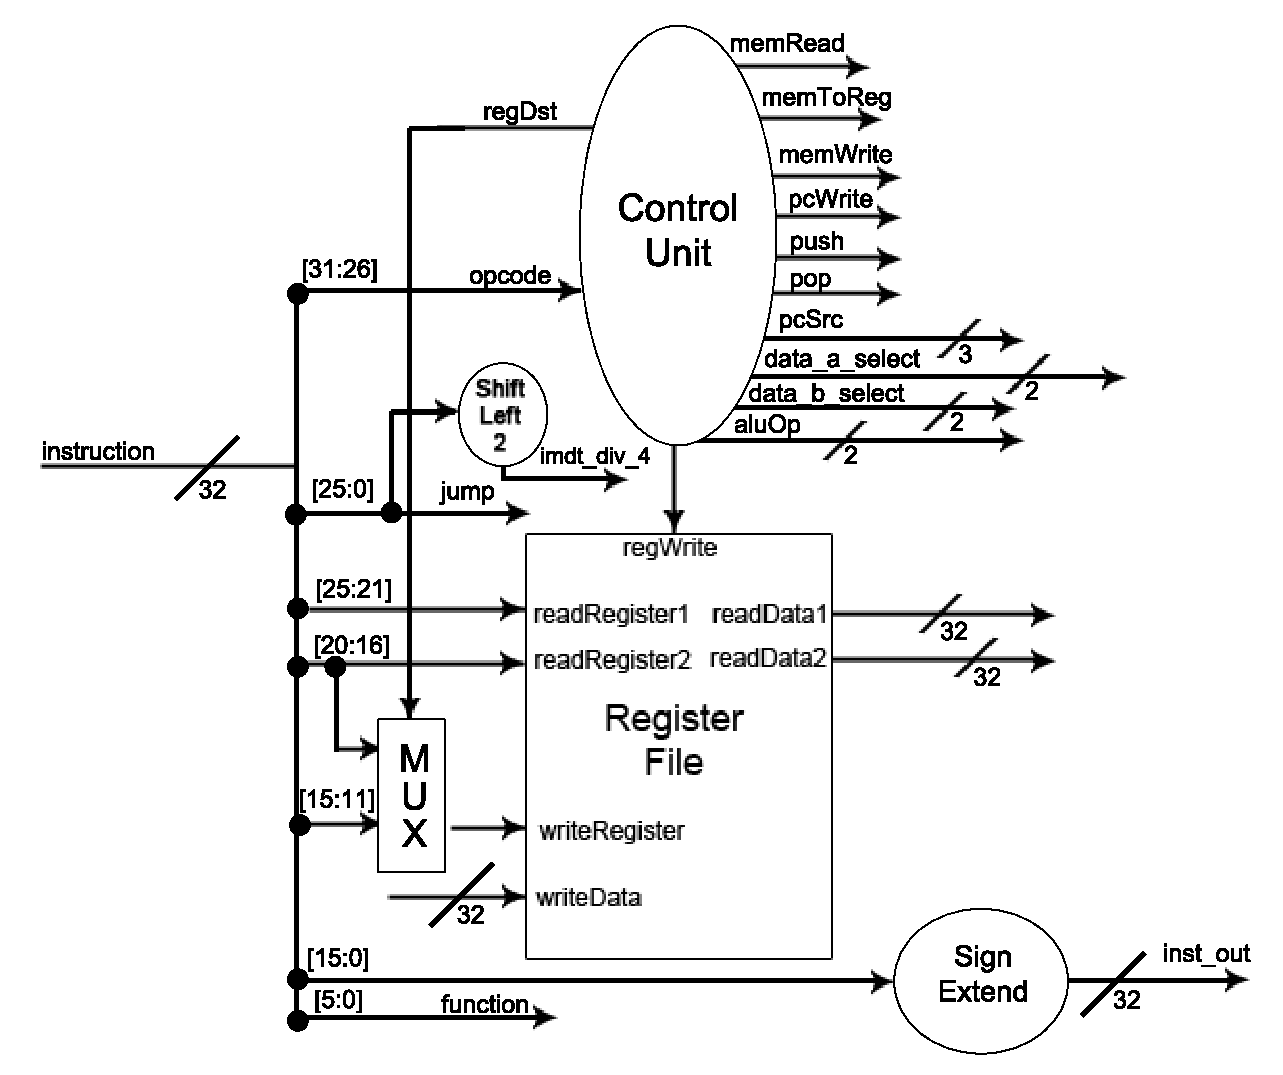
\includegraphics[scale=0.8]{./datapath/stage2.eps}
		\end{center}
	\end{figure}
